\documentclass[a4paper,12pt]{article}
\usepackage{graphicx}
\usepackage{fancyhdr}
\usepackage{listings}
\lstset
{
  numbers=left,
  breaklines=true,
}
\pagestyle{fancy}
\rhead{Dane Johnson}
\title{CS-456 Project 2}
\author{Dane Johnson}
\date{March 21st, 2018}
\headheight=15pt
\begin{document}
\maketitle
\newpage
\section{Motivation}

This project is meant to be a comparison of several different algorithms for finding All-Pairs-Shortest-Path.
The algorithms being compared are Floyd-Warshall, Johnson's using a Min-Priority Heap and Johnson's using a Fibonacci Heap. 

\section{Algorithms}
\subsection{Floyd-Warshall}
\subsubsection{Pseudocode}
\begin{lstlisting}[mathescape=true]
proc floyd-warshall(W)
  n $\gets$ W.rows
  D[0] $\gets$ W
  for k $\gets$ 1 to n
    D[k] $\gets$ new n$\times$n matrix
    for i $\gets$ 1 to n
      for j $\gets$ 1 to n
        $d[k]_{i,j}$ $\gets$ min($d[k-1]_{i,j}$, $d[k-1]{i,k}$ + $d[k-1]{k,j}$)
  return D[n] 
\end{lstlisting}
\subsubsection{Time Complexity}
This algorithm finds the shortest paths by iteratively constructing a 3d matrix. It must loop over every row of every column of every plane.
The dimensions are all based on V, so the time complexity is $\Theta(|V|^3)$.
\subsubsection{Correctness Proof}
\begin{description}
\item [Invariant: ] After the $k$th iteration, if the shortest path from a given $u$ to $v$ where $(u,v)\in E$ uses $k$ as an intermediate, $k$ will have been added to the path.
  from u to v
\item [Initialization: ] $k$ is 0 initially, a value not on the graph. Therefore no paths from $u$ to $v$ will pass through $k$.
\item [Maintenence: ] Two cases exist.
  \begin{enumerate}
  \item If using $k$ as an intermediate point on the path from $u$ to $v$ shortens the path, it is added to the path from $u$ to $v$.
  \item If using $k$ as an intermediate point on the path from $u$ to $v$ does not shorten the path, it is not added to the path from $u$ to $v$.
  \end{enumerate}
\item [Termination: ] When the loop terminates, $k = n$, so all intermediates will have been considered for all paths between vertices in the graph, and all shortest
  paths will have been selected.
\end{description}
\subsubsection{Empirical Validation}
\begin{figure}[h]
  \centering
  \textbf{Sparse Graph}\par\medskip
  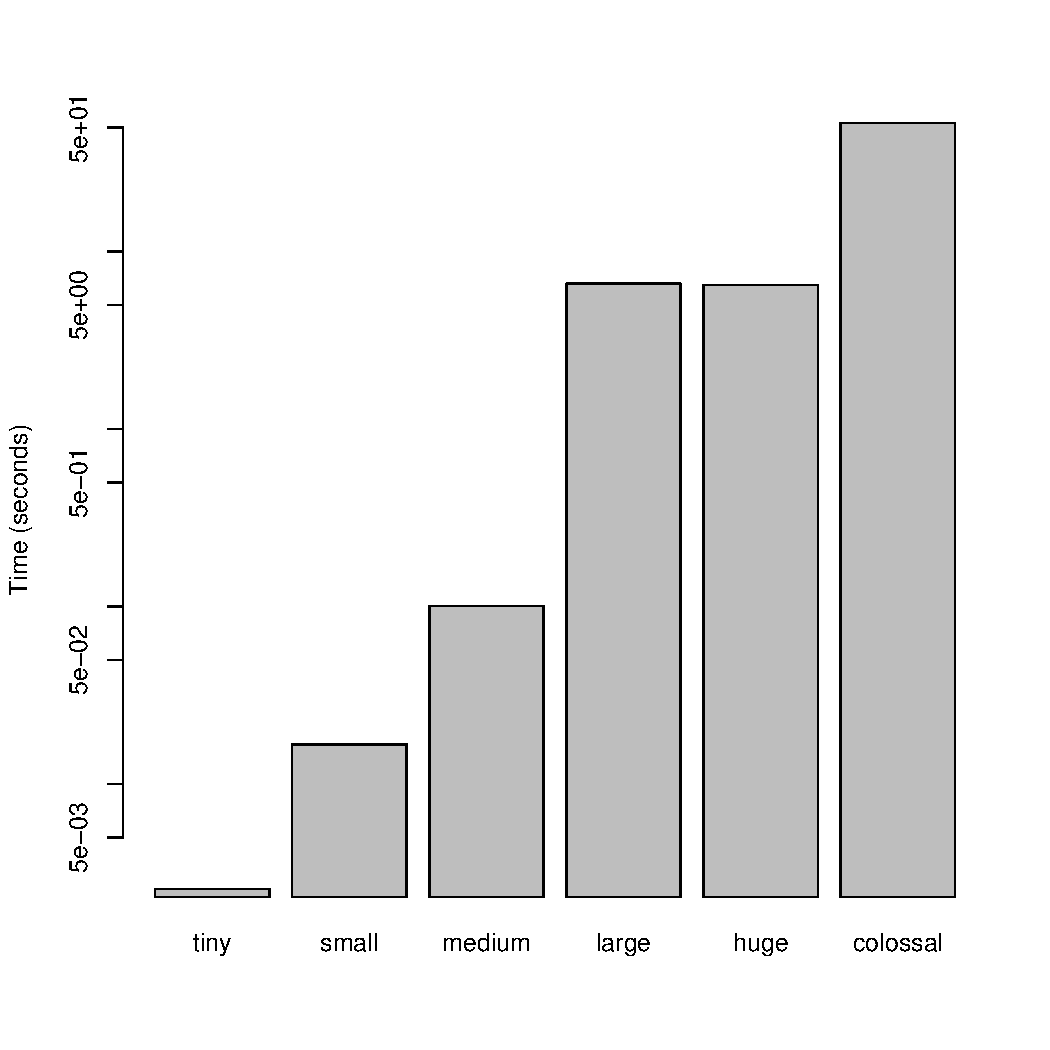
\includegraphics[scale=0.3]{Floyd-Warshallsparse}
\end{figure}
\begin{figure}[h]
  \centering
  \textbf{Dense Graph}\par\medskip
  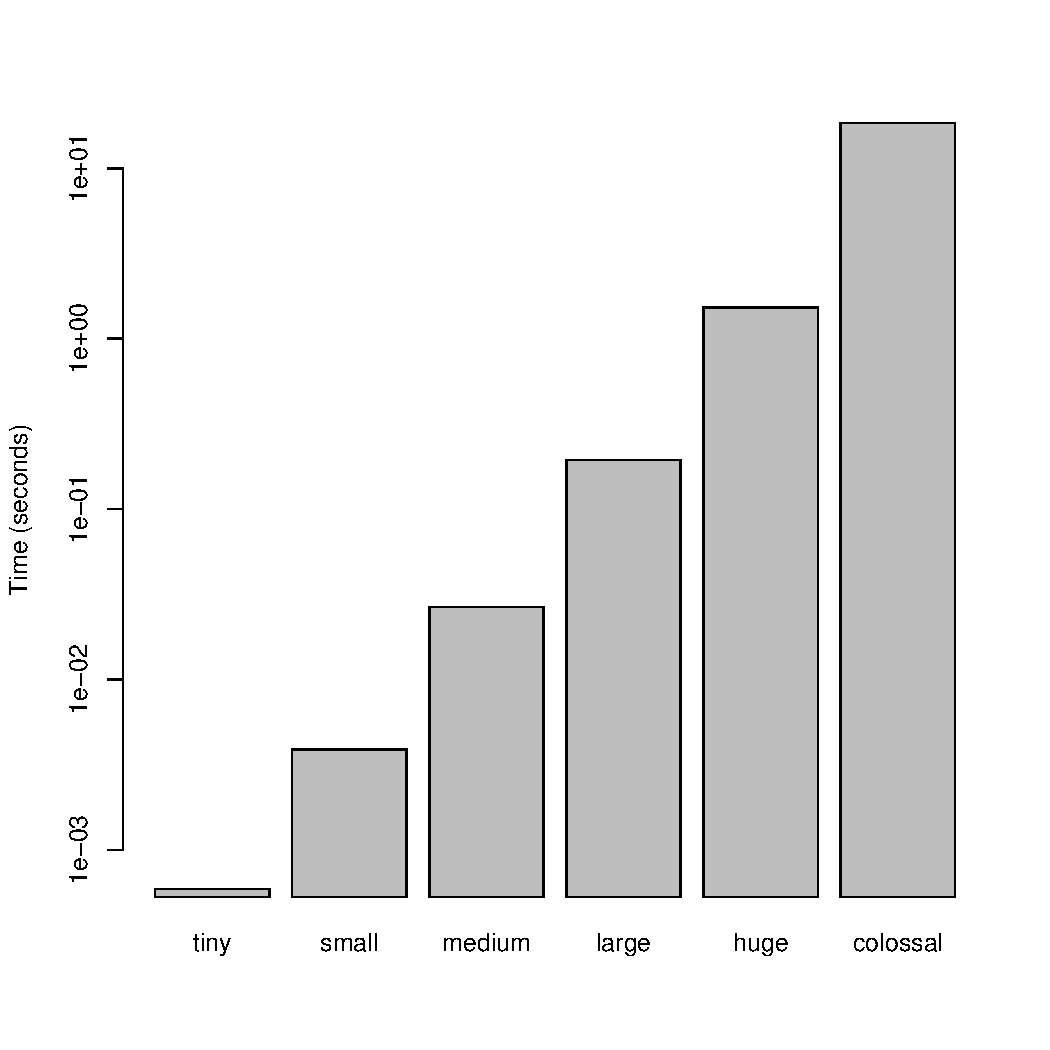
\includegraphics[scale=0.3]{Floyd-Warshalldense}
\end{figure}
\subsubsection{Observations}
\subsection{Djikstra's}
\subsubsection{Pseudocode}
\begin{lstlisting}[mathescape=true]
proc dijkstra(G, w, s)
  initialize-single-source(G, s)
  Q $\gets$ G.V
  while Q $\neq \emptyset$
    u $\gets$ extract-min(Q)
    for v $\in$ G.adj[u]
      relax(u, v, w)
\end{lstlisting}
\subsubsection{Time Complexity}
The initilization again takes $\Theta(|V|)$ time, exploring each vertex takes $V$ time, extracting a minimum takes $lg(V)$ time, and each edge is relaxed exactly once, $O(E)$ time. Therefore the runtime of the algorithm is based on what structure we choose to use for $Q$, which will be explored later, will cause the runtime to be either $O(Elg(V))$ if a Min Priority Heap is used, or $O(Vlg(V))$ if a Fibonacci Heap is used.
\subsubsection{Correctnesss Proof}
\begin{description}
\item [Invariant: ] At the start of each loop, the shortest path to every vertex that has been removed from $Q$ has been found.
\item [Initialization: ] Initially, no elements have been removed from $Q$, so the invariant is trivially proven.
\item [Maintenence: ] On each loop iteration, the number of explored elements is incremented, and by selecting the vertex closest to the source not in the explored space, we know that the shortest path to that vertex must be through its parent in the explored space.
\item [Termination: ] When the loop terminates, every vertex has been removed from $Q$, and by the invariant, the shortest path to every vertex is known.
\end{description}
\subsection{Johnson's}
\subsubsection{Pseudocode}
\begin{lstlisting}[mathescape=true]
proc johnsons(G, w)
  connect new node s with a weightless edge to every vertex $\forall v \in V$
  bellman-ford(G, w, s) // This will raise an error if there are negative weight cycles
  for $\forall v \in G.V$
    h(v) $\gets$ $\delta(s, v)$
  remove s from G
  for $\forall (u, v) \in G.E$
   $w'$(u, v) $\gets$ w(u, v) + h(u) - h(v)
  D $\gets$ V $\times$ V matrix
  for $\forall u \in G.V$
    run dijikstra(G, $w'$, u) to compute $\delta'(u, v) \forall v \in G.V$
    for $\forall v \in G.V$
      $d_{u,v}$ $\gets$ $\delta'(u, v)$ + h(v) - h(u)
  return D
\end{lstlisting}
\subsubsection{Time complexity}
The time complexity of connecting a new node is $\Theta(|V|)$, Bellman-Ford is $O(VE)$, removing the node is $\Theta(|V|)$, and creating the new weight function is $O(E)$. From here, we are updating every row of the new matrix, which has height $V$, by running Dijkstra's algorithm on each node. The time complexity of Dijkstra is depenedent on the data strucure in use, which will be explored later, if a Min Priority Heap is used, it will be $O(VElg(V))$, and it will be $O(V^2lg(V))$ if a Fibonnacci Heap is used.
\subsubsection{Correctness Proof}
\begin{description}
\item [Invariant: ] The shortest path from a source vertex $u$ to any vertex $v$ can be found by running Dijkstras algorithm on the reweighted graph, and then recalculating based on the original weight
\item [Initialization: ] Initially, no sources have been selected, so the shortest path of all selected elements is found trivially.
\item [Maintenence: ] On each loop iteration, Dijkstra's algorithm finds the shortest path to the reweighted edge, and then the shortest path to each vertex is found by recalculating based on the original graph weight.
\item [Termination: ] When the loop terminates, Dijkstra's algorithm has been run on every vertex, finding the shortest path to all other vertices. Therefore all pairs shortest paths have been found.
\end{description}
\subsection{Min Priority Heap}
\subsubsection{Code Walkthrough}
\lstinputlisting[language=Python, firstline=47, lastline=95]{shortestpath.py}
The Min Priority heap is implemented simply as a binary heap that maintains the heap
property on inserts and extractions. Decreasing a key, an operation that is done for every edge in Dijkstra, can at maximum climb from the furthest leaf to the root, and thus takes$O(lg(n))$ time. Extracting a min, which is done for every vertex in Dijkstra, must restore the heap property when a node is removed, which at worst moves an item from the root to the furthest leaf, which takes $O(lg(n))$ time. Finally, insertions involve a key decrease, taking the same amount of time. In Dijkstra, this is done for every vertex. However, when used in Dijkstra, the operation that is done the more is the key decrease, which is performed for each edge. Therefore, the runtime of Dijkstra using a Min Heap is $O(Elg(V))$.
\subsubsection{Empirical Validation}
\begin{figure}[h]
  \centering
  \textbf{Sparse Graph}\par\medskip
  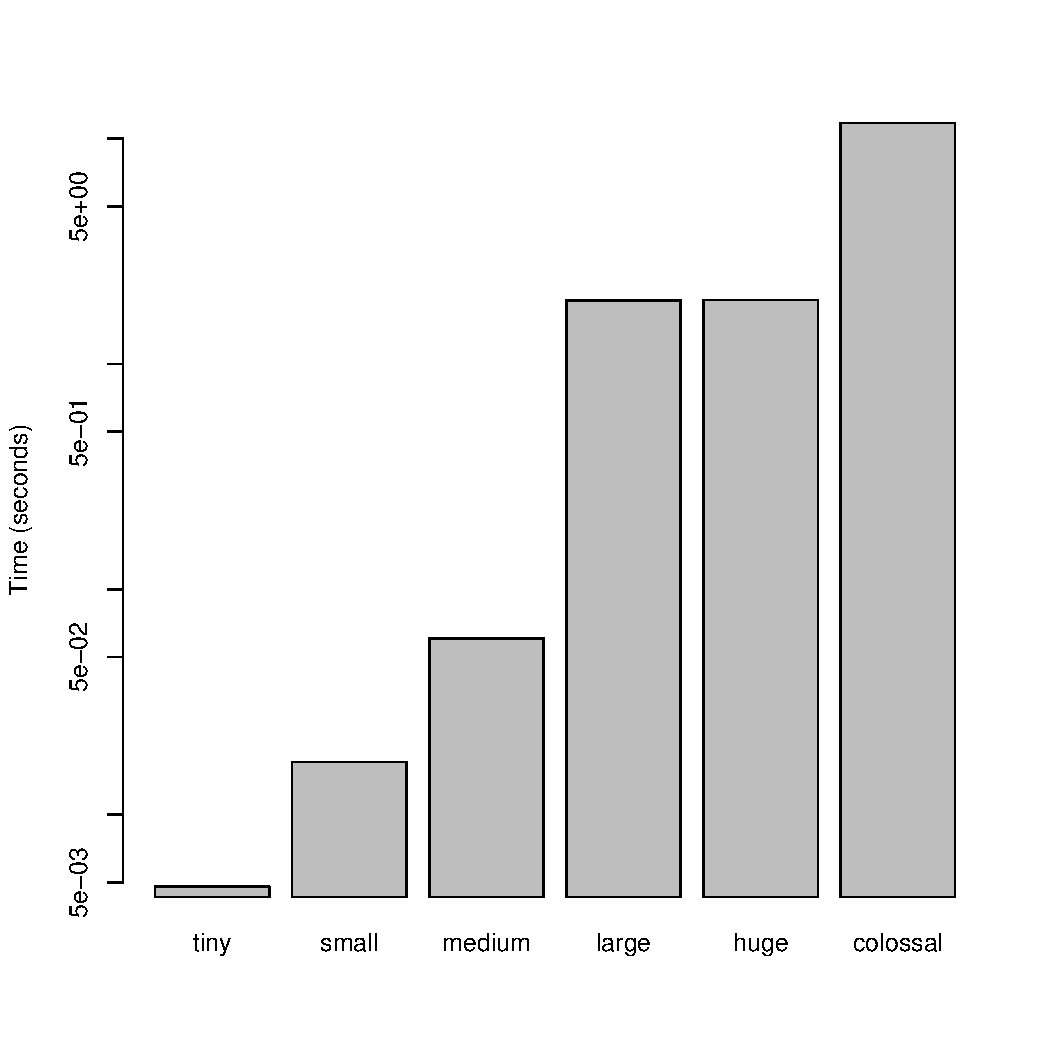
\includegraphics[scale=0.3]{Johnson-Min-Heapsparse}
\end{figure}
\begin{figure}[h]
  \centering
  \textbf{Dense Graph}\par\medskip
  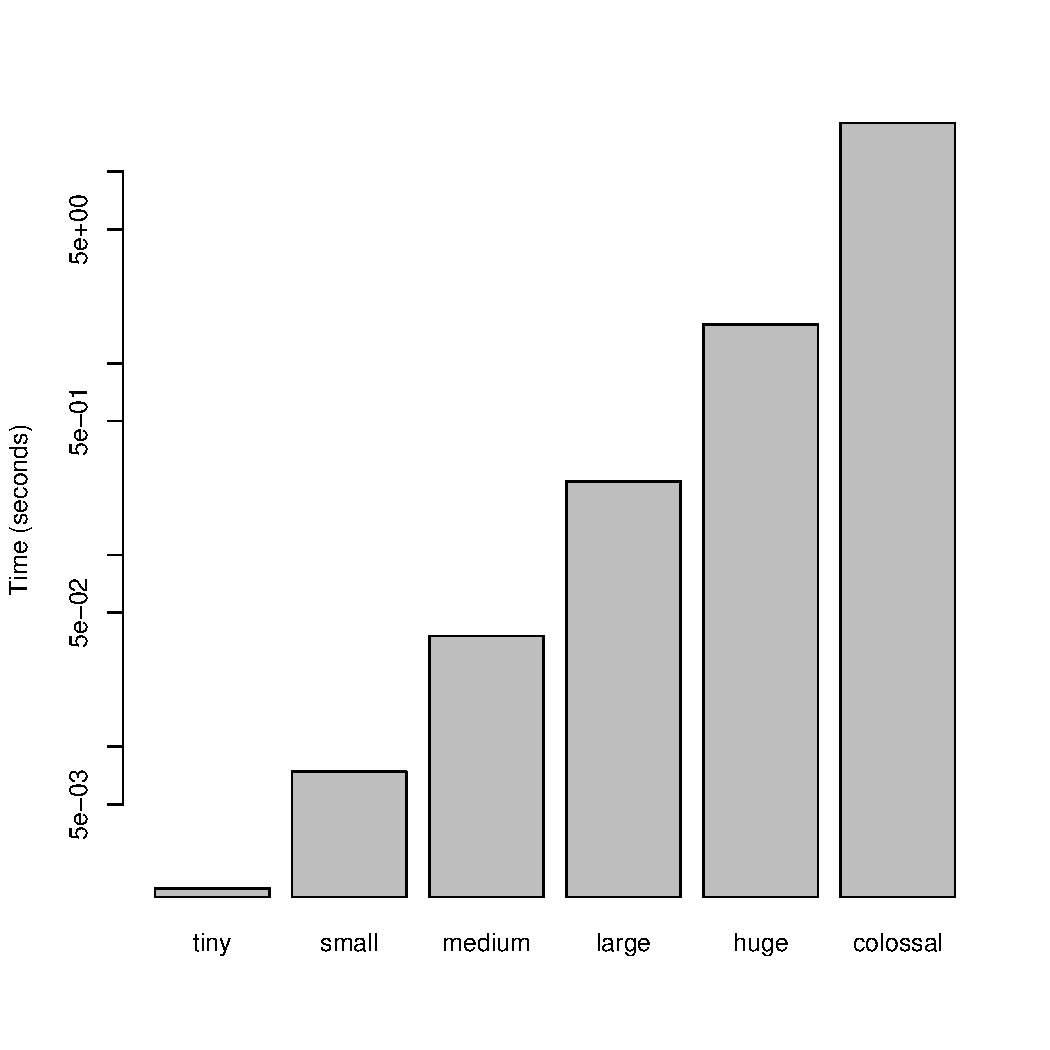
\includegraphics[scale=0.3]{Johnson-Min-Heapdense}
\end{figure}
\subsubsection{Observations}
\subsection{Fibonacci Heap}
\subsubsection{Code Walkthrough}
\lstinputlisting[language=Python, firstline=96, lastline=251]{shortestpath.py}
The Fibonacci Heap uses a mergeable heap structure. It maintains the heap structure only on extractions. Decreasing a key in a Fibonacci Heap involves cutting a branch and inserting it into the root, which is an $\Theta(1)$ constant time operation. Extracting a min involves rebuilding the heap structure, which can be performed in $O(lg(n))$ time. Finally, insertions can be done in $\Theta(1)$ constant time as well, as it simply involves inserting into a root list. Since the decrease-key operation can be done in constant time, this speeds up Dijkstra's algorithm, as the key decreases are no longer the limiting factor. The time complexity for Dijkstra with a Fibonacci Heap now is limited by the number of vertices next to the explored area, reducing the runtime to $O(V^2lg(V))$.
\subsubsection{Empirical Validation}
\begin{figure}[h]
  \centering
  \textbf{Sparse Graph}\par\medskip
  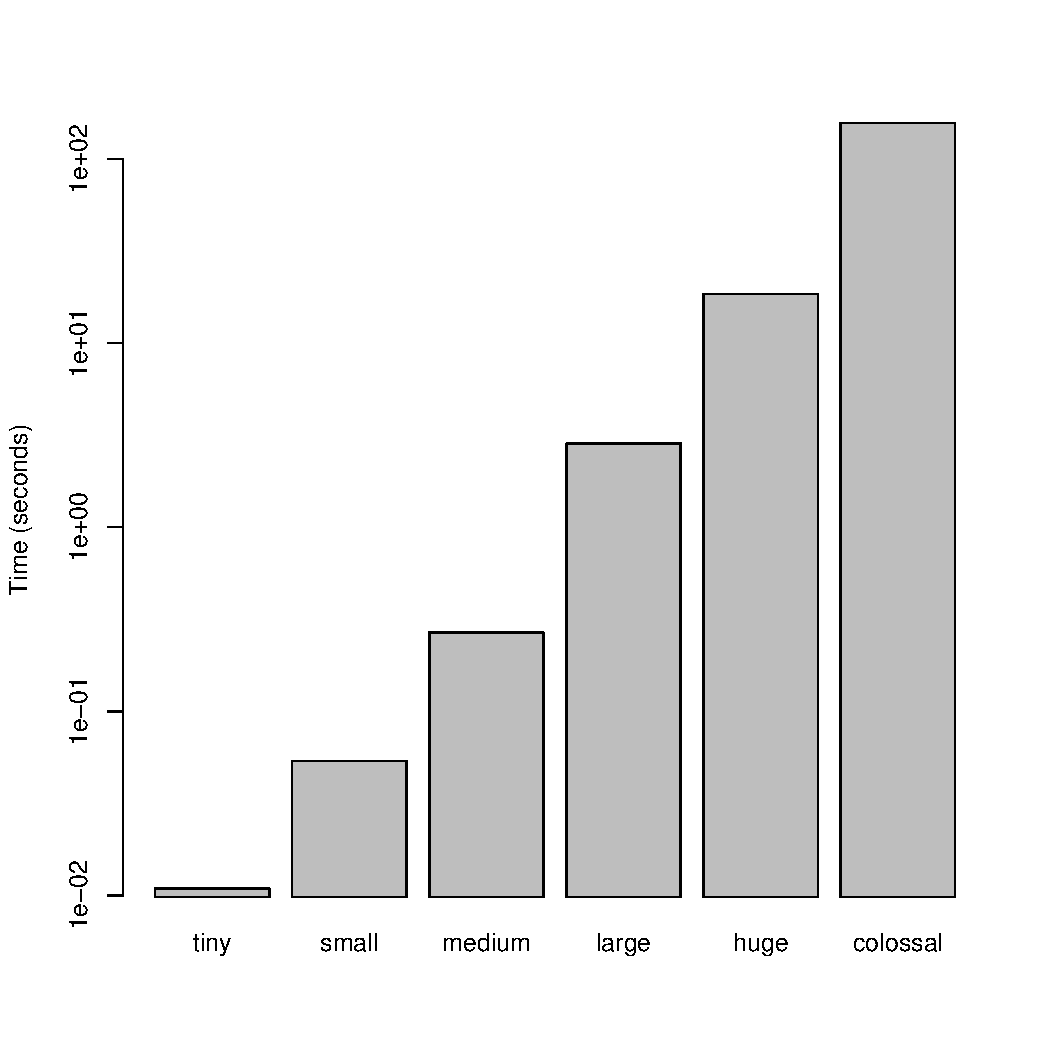
\includegraphics[scale=0.3]{Johnson-FibonacciHeapsparse}
\end{figure}
\begin{figure}[h]
  \centering
  \textbf{Dense Graph}\par\medskip
  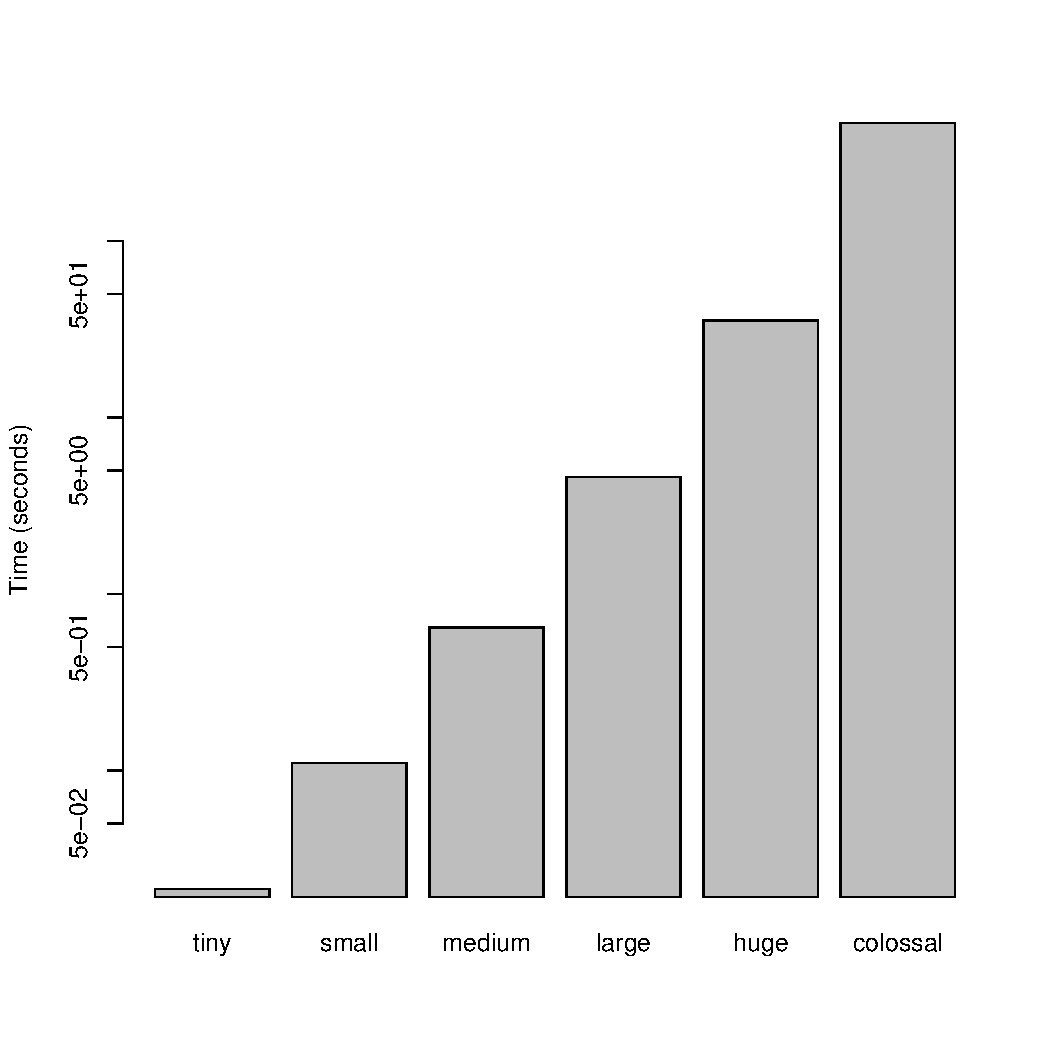
\includegraphics[scale=0.3]{Johnson-FibonacciHeapdense}
\end{figure}
\subsubsection{Observations}
\section{Conclusion}
\end{document}
